%%%%%%%%%%%%%%%%%%%%%%%%%%%%%%%%%%%%%%
% yale_thesis_alt.tex
% Robby Blum
% 2019/04/03
%
% A bare, sample template for a Yale PhD thesis using yalephd.cls
% This one has been modified from the regular version, in order to break up the content
% into multiple files that get inserted into the main one.
%%%%%%%%%%%%%%%%%%%%%%%%%%%%%%%%%%%%%%

\documentclass[letterpaper,12pt]{yalephd}
% remove draft option for final printing.
% font size must be between 10pt-12pt.

\usepackage{geometry} % you need this for yalephd.cls to work.
\usepackage{graphicx} % you probably want the rest of these.
\setkeys{Gin}{draft=false} % with this, basically all that the draft option does is add a header
\usepackage{dcolumn}
\usepackage{bm}
\usepackage{amsmath}
\usepackage{amsfonts}
\usepackage{amssymb}
\usepackage{appendix}
\usepackage{comment}
% If you're using BibLaTeX, you can't use the cite package, so comment it out (it's incompatible, but also redundant)
\usepackage{cite}
\usepackage{notoccite}
\usepackage[draft=false]{hyperref} % always generates hyperlinks, even in draft mode
\usepackage{cleveref}
% subcaption makes the hyperlinks to figures and such go to the top of the float, not the top of the caption.
% I assume it does other stuff as well, but that's why I used it.
\usepackage{subcaption}

% bibliography style if you're using BibTeX. Comment this out if using BibLaTeX!
\bibliographystyle{abbrvunsrt}

%% Load BibLaTeX if you're using it. These style options are similar to Physical Review Letters style,
%% but somewhat more verbose (titles are included, for instance).
%\usepackage[
%    backend=biber,
%    style=phys,
%    biblabel=brackets,
%    eprint=true
%]{biblatex}
%% If using BibLaTeX, you need to load your bibliography file in the preamble
%\addbibresource{name_of_your_bibtex_file.bib}


% Definitions file
\newcommand{\Pzero}{\widehat{P}_0}
% One space after periods, not two
\frenchspacing

% Need to define title before the abstract.
\title{Title goes here}
\author{Your name}
\advisor{Your advisor's name}
\date{Month, year you'll receive your degree, like ``May, 2015''} % usually not \today.

% This structure lets you remove parts of the document without changing the overall structure.
% So, if you comment out everything but chapter 2, the only material in the main text you get is
% chapter 2, but the page numbers, TOC, etc are all still correct. Useful for working on one part
% at a time.
\includeonly{
definitions,
content/1-introduction,
content/2-newchapter,
content/A-stuff,
content/B-morestuff
}

\begin{document}

% All the stuff at the front of your thesis.
\frontmatter

\begin{abstract}
	%% Add the text of your abstract here
Abstract goes here. Limit 750 words. This one has been inserted from another tex file: \texttt{content/0-abstract.tex}. % loads the abstract from a different file
	% this one uses \input bc it's just pasting text, but the chapters will use \include
\end{abstract}

\maketitle
\makecopyright{\printyear} % \printyear was populated from the \date{} entry already
\tableofcontents
\listoffigures % remove this if you have no figures.
\listoftables % remove this if you have no tables.


\chapter{Acknowledgements} % this needs to be before \mainmatter.
A lot of people are awesome. Probably your family, friends, 
advisor, and that one super special high school teacher who
believed in you.

% Starts proper arabic numbering of pages and chapters.
\mainmatter

%% Include your chapters here
\chapter{Introduction} \label{chapter1}
Your first chapter is probably an introduction. But who knows. Check out Eq.\ (\ref{that_right_triangle_rule})!
Note that after Eq.\ and Fig.\ you want to use `.\textbackslash'  to use a single sized space. Otherwise,
latex will interpret it as the end of a sentence and put additional white space in between `Eq.' and 
`(\ref{that_right_triangle_rule})'.
Actually, you might want to input a tilde (\texttt{\~}) (a non-breaking space) instead of a space, so that the `Eq.' and number don't break across a line.
Or you could use commands from \texttt{hyperref} or \texttt{cleveref}.
See \cref{chapter2} for that...

By the way, I strongly recommend splitting up your paragraphs so that you have each sentence on its own line.
This makes the diffs much easier to read, which makes version control more useful.

\begin{equation}
a^2 + b^2 = c^2 \label{that_right_triangle_rule}
\end{equation}

The Physics Department recommends that the first chapter of the thesis be 
a succinct summary of the entire thesis, including in particular:

\begin{enumerate}
  \item a brief review of the field prior to the thesis research to provide context
  \item a presentation of the goals and motivations of the thesis research 
  \item a clear description of what the student has achieved in the thesis research
 (primarily written in the first person singular, but with due credit to
 others as appropriate). This description should refer back to (1) and clearly indicate the relation
 to prior work.
\end{enumerate}
It may also make sense to add suggestions for how to best build upon the thesis research in future work. Otherwise these suggestions should appear in the conclusion of the thesis.


\chapter{A new chapter}
Your second chapter probably has novel material in it. hopefully. Here's a math object written using a shortcut that I defined in a separate file: $\Pzero$.

% Add additional \chapter{}s as necessary.

% use \cite{} to cite a reference in your bibliography file.
% use \ref{} to reference a \label{} from an equation, figure, or table.

% for sets of equations use align or gather:
%\begin{align}
%\end{align}

% for long equations, use multline.

% for figures:
\begin{figure}[ht]
\centering
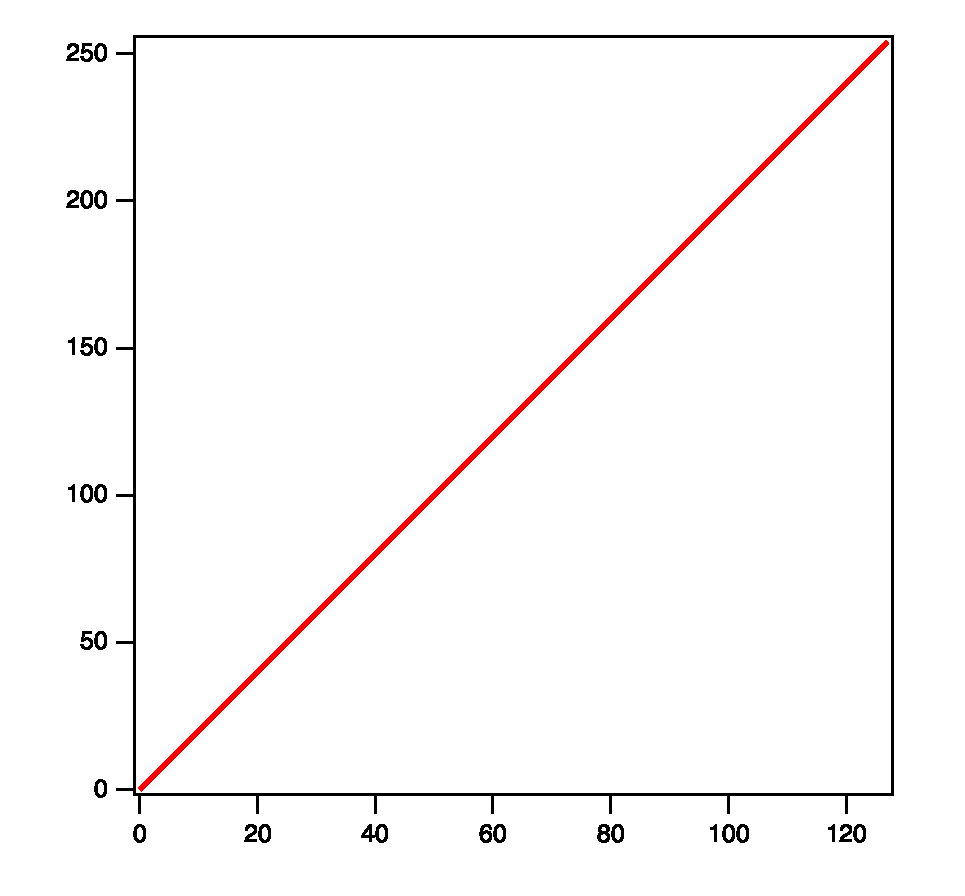
\includegraphics[width=.45\textwidth]{name_of_figure.eps}
\caption{A caption! \label{a_figure}}
\end{figure}

% for tables:
\begin{table}
\centering
\begin{tabular}{c|c|c}
 1 & 2 & 3 \\
\hline
\end{tabular}
\caption{Another caption! \label{a_table}}
\end{table}



% once you're finished your main chapters, on to the appendices
% Only call appendix once, here.
\appendix

\chapter{Stuff}
If you need an appendix, it will go here.

\begin{align}
a^n + b^n &\ne c^n \\
n &> 2
\end{align}

\chapter{More stuff}
A second appendix. Look at you, you over achiever.

% Any chapters such as End Notes go after this.
\backmatter

% for your own sake, use a bibtex file, so all of the numbering of references will be done
% automatically. BibTeX version:
\bibliography{name_of_your_bibtex_file}
% BibLaTeX version:
%\printbibliography[heading=bibintoc]

\end{document}
